% --------------------------------------------------------------
% This is all preamble stuff that you don't have to worry about.
% Head down to where it says "Start here"
% --------------------------------------------------------------
 
\documentclass[12pt]{article}
 
\usepackage[margin=1in]{geometry} 
\usepackage{amsmath,amsthm,amssymb,listings,xcolor,graphicx,framed,subfig}
\usepackage{booktabs}
\usepackage{gensymb}

\newcommand{\N}{\mathbb{N}}
\newcommand{\Z}{\mathbb{Z}}
 
\newenvironment{theorem}[2][Theorem]{\begin{trivlist}
\item[\hskip \labelsep {\bfseries #1}\hskip \labelsep {\bfseries #2.}]}{\end{trivlist}}
\newenvironment{lemma}[2][Lemma]{\begin{trivlist}
\item[\hskip \labelsep {\bfseries #1}\hskip \labelsep {\bfseries #2.}]}{\end{trivlist}}
\newenvironment{exercise}[2][Exercise]{\begin{trivlist}
\item[\hskip \labelsep {\bfseries #1}\hskip \labelsep {\bfseries #2.}]}{\end{trivlist}}
\newenvironment{problem}[2][Problem]{\begin{trivlist}
\item[\hskip \labelsep {\bfseries #1}\hskip \labelsep {\bfseries #2.}]}{\end{trivlist}}
\newenvironment{question}[2][Question]{\begin{trivlist}
\item[\hskip \labelsep {\bfseries #1}\hskip \labelsep {\bfseries #2.}]}{\end{trivlist}}
\newenvironment{corollary}[2][Corollary]{\begin{trivlist}
\item[\hskip \labelsep {\bfseries #1}\hskip \labelsep {\bfseries #2.}]}{\end{trivlist}}

\newenvironment{solution}{\begin{proof}[Solution]}{\end{proof}}

\definecolor{codegreen}{rgb}{0,0.6,0}
\definecolor{codegray}{rgb}{0.5,0.5,0.5}
\definecolor{codepurple}{rgb}{0.58,0,0.82}
\definecolor{backcolour}{rgb}{0.97,0.97,0.97}
\lstdefinestyle{pystyle}{
    backgroundcolor=\color{backcolour},   
    commentstyle=\color{codegreen},
    keywordstyle=\color{magenta},
    numberstyle=\tiny\color{codegray},
    stringstyle=\color{codepurple},
    basicstyle=\ttfamily\tiny\tiny,
    breakatwhitespace=false,         
    breaklines=true,                 
    captionpos=b,                    
    keepspaces=true,                 
    numbers=left,                    
    numbersep=5pt,                  
    showspaces=false,                
    showstringspaces=false,
    showtabs=false,                  
    tabsize=2
}
\lstset{style=pystyle}

\graphicspath{{./figures}}
 
\begin{document}
 
\title{Homework 1: Georgiatenna}
\author{Matthew Luyten\\ %replace with your name
ECE8803}

\maketitle

\begin{enumerate} 
    \item[I.] Results
    
    \begin{figure}[!ht]
        \centering
        
\includegraphics[width=5.5in]{ga_coverage.eps}
        \caption{-80 dBm Coverage Map}
    \end{figure}

    \begin{table}[h!]
        \centering
        \begin{tabular}{c c c} 
            \toprule
            Coverage Above -80 dBm & 259,360 $\text{km}^2$ & 255,458 pixels\\
            Coverage Above -80 dBm Outside Georgia & 99,673 $\text{km}^2$ & 100,261 pixels\\
            Coverage Above -83 dBm & 65,700 $\text{km}^2$ &\\
            \bottomrule
        \end{tabular}
        \caption{Design Results}
        \label{table:1}
    \end{table}
    
    \begin{table}[h!]
        \centering
        \begin{tabular}{c c } 
            \toprule
            Satellite Longitude & -75.5\degree \\
            Boresight Pointing Locaiton & (-83.6\degree, 32.8\degree) \\ 
            Array Size & 150$\times$150 \\
            Active Elements & 6040 \\
            Uniform Phase Taper & 0\degree \\
            Peak $|\text{AF}|^2$ & 75.62 dB \\
            Transmit Power & 42.734 dBm \\
            \bottomrule
        \end{tabular}
        \caption{Design Parameters}
        \label{table:1}
    \end{table}

    \begin{figure}[!ht]
        \subfloat[]{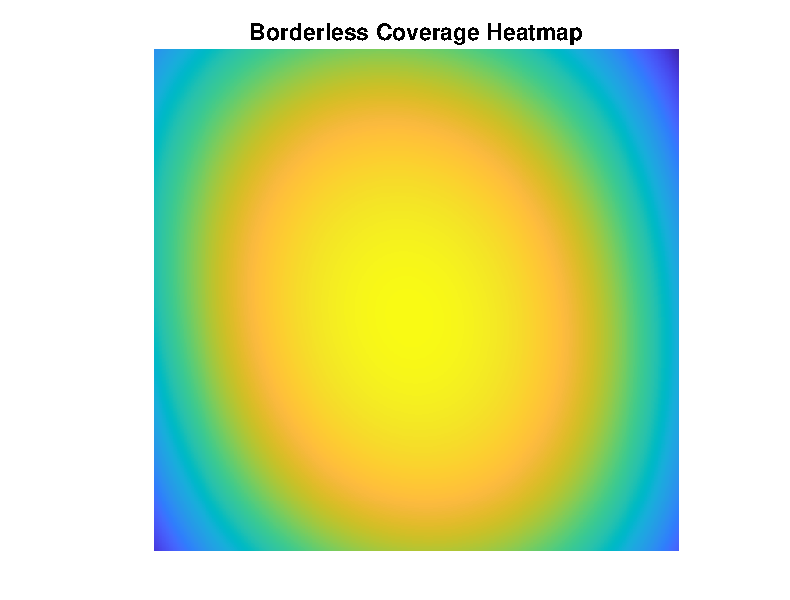
\includegraphics[width=3.2in]{borderless_heatmap.eps}}
        \subfloat[]{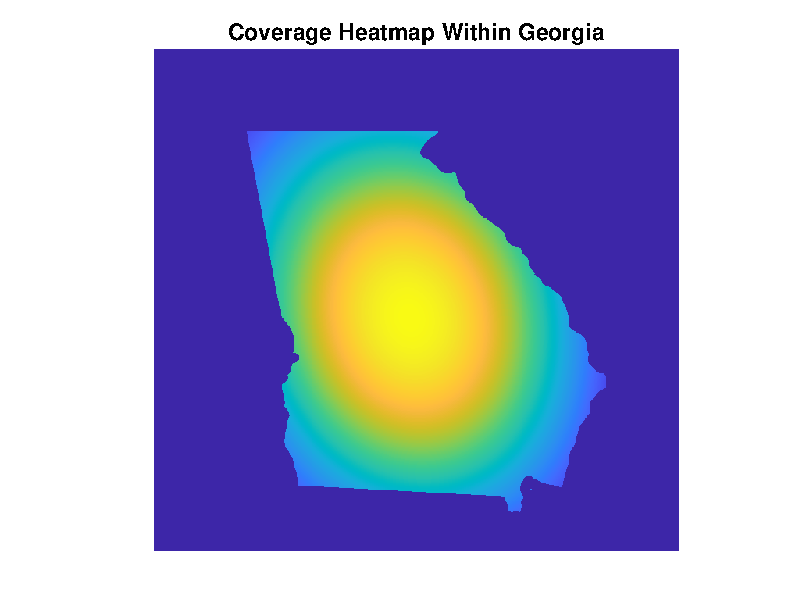
\includegraphics[width=3.2in]{ga_heatmap.eps}}
        \caption{Coverage Heatmaps}
        \centering
    \end{figure}

    \begin{figure}[!ht]
        \subfloat[]{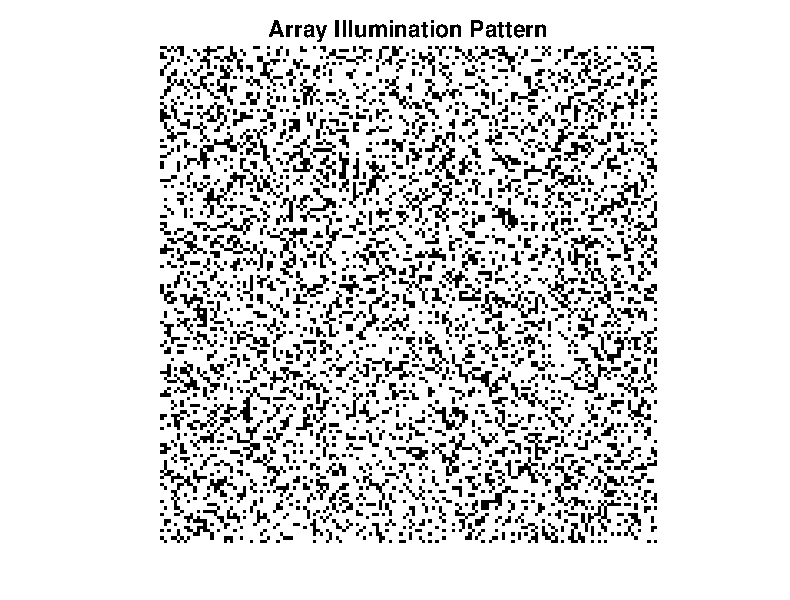
\includegraphics[width=3.2in]{arr_pattern.eps}}
        \subfloat[]{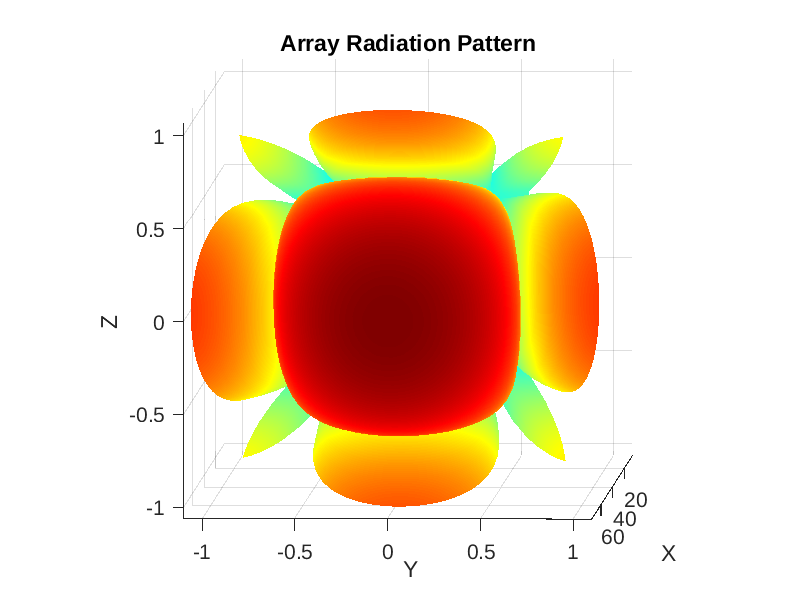
\includegraphics[width=3.2in]{rad_pattern.eps}}
        \caption{Antenna Characteristics}
        \centering
    \end{figure}

    \newpage
    \hphantom{}
    \newpage

    \item[II.] Design Methodology
    
    This solution was determined by utilizing a genetic algorithm. The original generation (20 patterns)
    is determined by randomly setting the value of each element to on or off. Each pattern is then scored
    according to the following formula:

    \[\text{Exclusion Rate} = 
    \frac{\text{Pixels Below Avg. Power Outside GA}}{\text{Pixels Outside GA}}\]

    \[\text{Inclusion Rate} = 
    \frac{\text{Pixels Below Avg. Power Inside GA}}{\text{Pixels Inside GA}}\]

    \[\text{Score} = 60 \times \text{Exclusion Rate} + 40 \times \text{Inclusion Rate}\]

    The best 10 patterns are kept and the other 10 patterns are created by element-wise ANDing the top 10
    patterns with one another. Finally, all patterns are mutated by randomly flipping a few bits.
    This is performed over 500 iterations. If no new optimal solutions are found for 100 consecutive
    iterations, a new population is created at random.

    The pattern with the best score is then analyzed to determine the required transmit power 
    to maximize exclusionary coverage. 

    \item[II.] Code
    
    \begin{lstlisting}[language=matlab]
function [r, el, az] = transformSatOrigin(obs_lat, obs_lon, sat_lat, sat_lon, r_sat)
    re = 6.378e6;

    r_x = r_sat - (re .* sin((pi/2)-obs_lat) .* cos(obs_lon-sat_lon));
    r_y = -re .* sin((pi/2)-obs_lat) .* sin(obs_lon-sat_lon);
    r_z = re .* cos((pi/2)-obs_lat);
    
    r = sqrt(r_x.^2 + r_y.^2 + r_z.^2);
    az = atan(r_y ./ r_x);
    el = acos(r_z ./ r);
end
    \end{lstlisting}

    \begin{lstlisting}[language=matlab]
function af = arrayFactor(ant_array, beta, theta, phi)
    r_hat_x = sin(theta) .* cos(phi);
    r_hat_y = sin(theta) .* sin(phi);
    r_hat_z = cos(theta);

    [M, N] = size(ant_array);
    af = zeros(size(theta));
    for y = 0:1:N-1
        for z = 0:1:M-1
            if ant_array(z+1, y+1) > 0
                r_dot_r_hat = r_hat_y * y + r_hat_z * z;
                af = af + ant_array(z+1, y+1) * exp(-1i * (pi * r_dot_r_hat + beta));
            end
        end
    end
    af = abs(af);
end
    \end{lstlisting}

    \begin{lstlisting}[language=matlab]
function rx_power = calcReceivePower(rx_gain, tx_gain, tx_power, k, distance)
    path_loss = 20 * log10(k * distance);
    rx_power = tx_power + tx_gain + rx_gain - path_loss;
end
    \end{lstlisting}

    \begin{lstlisting}[language=matlab]
function plotRadiationPattern(array, N)
    [Theta, Phi] = meshgrid(linspace(91*pi/180, 89*pi/180, N), ...
        linspace(-1*pi/180, 1*pi/180, N));
    af = arrayFactor(array, 0, Theta, Phi);
    r = 20*log10(af);
    
    % Convert spherical to Cartesian coordinates
    X = r .* sin(Theta) .* cos(Phi);
    Y = r .* sin(Theta) .* sin(Phi);
    Z = r .* cos(Theta);
    
    % Create the spherical surface plot
    surf(X, Y, Z, r);
    
    % Customize the plot
    title('Radiation Pattern');
    xlabel('X'); ylabel('Y'); zlabel('Z');
    axis equal;
    colormap jet;
    shading interp;
end
    \end{lstlisting}

    \begin{lstlisting}[language=matlab]
function plotMaskedHeatmap(data, mask)
    data = data .* mask;
    data = max(data - min(data(data ~= 0)), 0);
    data = data * 223 / max(data, [], "all");
    data = (data + 32) .* mask;
    imagesc(data); axis equal; axis off;
end
    \end{lstlisting}

    \begin{lstlisting}
function new_pop = nextGeneration(pop, scores)
    mutation_q = 0.75;
    [~, ~, N] = size(pop);
    [~, idx] = sort(scores, "descend");
    pop = pop(:, :, idx);
    new_pop = pop;
    
    idx = N/2;
    for mother = 1:N/2
        for father = mother+1:N/2
            new_pop(:, :, idx) = pop(:, :, mother) & pop(:, :, father);
            idx = idx + 1;
            if idx > N
                break;
            end
        end
        if idx > N
            break;
        end
    end

    mutations = randn(size(new_pop)) > mutation_q;
    new_pop = (new_pop & ~mutations) | (~new_pop & mutations);
end
    \end{lstlisting}

    \begin{lstlisting}[language=matlab]
load("GAmap.mat");
r_sat = 42.400e6;
freq = 30e9;
k = 2 * pi / (3e8 / freq);
tx_power = 60;
rx_gain = 10;

% Array dimensions
R_arr = 150;
C_arr = 150;

% Number of patterns in population
pop_sz = 20;

sat_lat = 0 * pi / 180;
sat_lon = -75.5* pi / 180;

bs_lat = 32.8 * pi / 180;
bs_lon = -83.6 * pi / 180;

[~, bs_el, bs_az] = transformSatOrigin(bs_lat, bs_lon, sat_lat, sat_lon, r_sat);

[rows, cols] = size(GA.data);

data = GA.data(1:10:rows, 1:10:cols) > 128;
lats = GA.lat(1:10:rows, 1:10:cols) * -1 * pi / 180;
lons = GA.lon(1:10:rows, 1:10:cols) * pi / 180; 

[dist, el, az] = transformSatOrigin(lats, lons, sat_lat, sat_lon, r_sat);
el = el - bs_el + pi/2;
az = az - bs_az;

array_pop = randn(R_arr, C_arr, pop_sz) > 0.15;

scores = zeros(1, pop_sz);
avgs = zeros(1, pop_sz);
sol = zeros(R_arr, C_arr);
sol_score = 0;

[M_lat, N_lon] = size(el);
[M, N, ~] = size(array_pop);
[z, y] = meshgrid(0:1:M-1, 0:1:N-1);
r_hat_y = reshape(sin(el) .* sin(az), 1, M_lat * N_lon);
r_hat_z = reshape(cos(el), 1, M_lat * N_lon);
z = reshape(z, 1, M*N)';
y = reshape(y, 1, M*N)';
exp_term = exp(-1i * pi * (y * r_hat_y + z * r_hat_z));
clear z;
clear y;
clear r_hat_z;
clear r_hat_y;

duds = 0;

for i = 1:500
    for j = 1:pop_sz
        a = reshape(array_pop(:, :, j), 1, M*N);
        tx_gain = 10*log10(2 * reshape(abs(a * exp_term), M_lat, N_lon).^2); % 2 = directivity/gain of half-space radiating element
        rx_power = calcReceivePower(rx_gain, tx_gain, tx_power, k, dist);
        avg = mean2(rx_power) * 0.9995;
        exclusion_rate = sum((rx_power < avg) .* (data < 1) , "all") / sum(data < 1, "all");
        inclusion_rate = sum((rx_power >= avg) .* data, "all") / sum(data, "all");
        scores(j) = 60*exclusion_rate + 40*inclusion_rate;
        count = j + (i-1) * pop_sz;
    end
    
    if max(scores) > sol_score
        [sol_score, idx] = max(scores)
        sol = array_pop(:, :, idx)
        duds = 0;
    else
        duds = duds + 1;
    end
    
    if (duds > 100)
        array_pop = randn(R_arr, C_arr, pop_sz) > 0.15;
        duds = 0;
    else
        array_pop = nextGeneration(array_pop, scores);
    end
end

solution = struct;
solution.array = sol;
save("solution.mat", "solution");

clear exp_term; % This term is huge
    \end{lstlisting}

    \begin{lstlisting}
% -------------- SET UP ENVIRONMENT --------------
load("solution.mat");
sol = solution.array;
load("GAmap.mat");

r_sat = 42.400e6;
freq = 30e9;
k = 2 * pi / (3e8 / freq);
tx_power = 45.744338999144280;
rx_gain = 10;

sat_lat = 0 * pi / 180;
sat_lon = -75.5* pi / 180;

bs_lat = 32.8 * pi / 180;
bs_lon = -83.6 * pi / 180;

[~, bs_el, bs_az] = transformSatOrigin(bs_lat, bs_lon, sat_lat, sat_lon, r_sat);

data = GA.data > 128;

lats = GA.lat * -1 * pi / 180;
lons = GA.lon * pi / 180; 

[dist, el, az] = transformSatOrigin(lats, lons, sat_lat, sat_lon, r_sat);
el = el - bs_el + pi/2;
az = az - bs_az;

% -------------- FIND RX POWER ACROSS MAP --------------

tx_gain = 10*log10(2 * arrayFactor(sol, 0, el, az).^2); % 2 = directivity/gain of half-space radiating element
rx_power = calcReceivePower(rx_gain, tx_gain, tx_power, k, dist);
avg = mean2(rx_power) * 0.99975;

% -------------- DETERMINE POWER THRESHOLD --------------

opt_score = 0;
opt_thresh = 0;

for scale = linspace(min(rx_power, [], "all"), max(rx_power, [], "all"), 100)
    thresh = scale;
    exclusion_rate = sum((rx_power < thresh) .* (data < 1) , "all") / sum(data < 1, "all");
    inclusion_rate = sum((rx_power >= thresh) .* data, "all") / sum(data, "all");
    score = 100*exclusion_rate*(inclusion_rate > 0.999);
    if opt_score < score
        opt_score = score;
        opt_thresh = thresh;
    end
end

req_power = tx_power + (-80 - opt_thresh)

lat_delta = abs(lats(1,1)-lats(2,1)) * 180 / pi * 111.1;
lon_delta = abs(lons(1,1)-lons(1,2)) * 180 / pi * cos(mean2(lats)) * 111.1;
cell_area = lat_delta * lon_delta;

area_80db = sum((rx_power > opt_thresh), "all") * cell_area
non_excluded_area = sum((rx_power > opt_thresh) .* (data < 1) , "all") * cell_area
area_83db = sum((rx_power > opt_thresh+3) .* data, "all") * cell_area
af_peak = 20*log10(arrayFactor(sol, 0, pi/2, 0))
active_elements = sum(sol, "all")

pixels_80db = sum((rx_power > opt_thresh), "all")
non_excluded_pixels = sum((rx_power > opt_thresh) .* (data < 1) , "all")

rx_power_within = sum(10.^(rx_power/10) .* data, "all")
rx_power_without = sum(10.^(rx_power/10) .* (data < 1), "all")

% -------------- PLOT FIGURES --------------

figure(1);
plotRadiationPattern(sol, 50);
title("Array Radiation Pattern");

view([90.18 0.28])

figure(2);

imagesc(sol*-1);
axis equal; axis off;
colormap gray;
set(gca,'LooseInset',get(gca,'TightInset'));
title("Array Illumination Pattern");

figure(3);
imagesc(rx_power); axis equal; axis off;
title("Borderless Coverage Heatmap");
set(gca,'LooseInset',get(gca,'TightInset'));
colormap parula;

figure(4);
plotMaskedHeatmap(10.^(rx_power/10), data);
title("Coverage Heatmap Within Georgia");
set(gca,'LooseInset',get(gca,'TightInset'));
colormap parula;

figure(5);
imagesc(2 * (rx_power > opt_thresh) + data); axis equal; axis off;
title("Georgia Coverage above -80 dBm");
set(gca,'LooseInset',get(gca,'TightInset'));
clear exp_term;
colormap jet;

solution = struct;
solution.array = sol;
solution.rx_power = rx_power;
solution.coverage = rx_power > -80;
save("solution.mat", "solution");
    \end{lstlisting}

\end{enumerate}

\end{document}